\subsection{Derivate Parziali}

\subsubsection{Derivate parziali per n=1}

nel caso reale: \(f: I \subset \R \to \R \) con \(x \mapsto f(x)\)

\(f'(x_0)\) è il limite di:

\[
    \lim_{ h \to 0 } \frac{f(x_0+h)-f(x_0)}{h}
\]

se esiste ed è finito, questo limite misura il tasso di variazione istantanea di \(f\) nel punto \(x_0\).

Quindi \(f'(x_0)\) rappresenta la pendenza della retta tangente al grafico \(f\) nel punto \(p_0=(x_0,f(x_0))\)

\subsubsection{Derivate parziali per n=2}

Sia \(f: \R^2 \to \R \) e \(P_0=(x_0,y_0)\)

Adesso diventa importante come mi sposto per arrivare a \(x_0\) avendo più gradi di movimento intorno a \(x_0\).

Vogliamo calcolare la derivata parziale di \(f\) fatta rispetto a \(x\) in \((x_0,y_0)\):

\[
    \lim_{ h \to 0 } \frac{f(x_0+h,y_0) -f(x_0,y_0)}{h}
\]

purché esista, finito.

Anche la derivata parziale di \(f\) rispetto ad \(y\) nel punto \((x_0,y_0)\):

\[
    \lim_{ h \to 0 } \frac{f(x_0,y_0+h) - f(x_0,y_0)}{h}
\]

purché esista, finito.

Queste due derivate si indicano:

\[
    \frac{\partial f}{\partial x}(x_0,y_0) = f_x(x_0,y_0) = D_{x}f(x_0,y_0)
\]

\[
    \frac{\partial f}{\partial y}(x_0,y_0) = f_y(x_0,y_0)= D_{y}f(x_0,y_0)
\]

\filbreak{}
\subsubsection{Derivate parziali per n generico}

\begin{align*}
    f: A \subseteq \Rn & \to \R \qquad \text{con A definito} \\
    \ux                & \mapsto f(\ux)
\end{align*}
Sia \(P_0= (x_1, \ldots, x_{i}, \ldots, x_n) \in A\)

Si definisce \textbf{derivata parziale di \(f\) fatta rispetto a \(x_i\) nel punto \(P_0=(x_1, \ldots ,x_n)\)}, il limite:

\[
    \lim_{ h \to 0 } \frac{f(x_1,\ldots,x_{i-1},x_{i}+h,x_{i+1},\ldots,x_n) - f(x_1,\ldots,x_{i},\ldots,x_n)}{h}
\]

se esiste ed è finito. Questo limite si indica nei seguenti modi:
\begin{align*}
    \frac{\partial f}{\partial x_{i}}(\ux) &  & D_{x_{i}}f(\ux) &  & f_{x_{i}}(\ux)
\end{align*}

\filbreak{}
\subsubsection{Metodo delle tracce (n=2)}

Vediamo come calcolare:

\[
    f_x(x_0,y_0) ,\  f_y(x_0,y_0)
\]

Per la derivata parziale rispetto a \(x\) nel punto \(P_0=(x_0,y_0)\), tengo fermo \(y=y_0\) e derivo rispetto a \(x\):

\[
    g_1(x)= f(x,y_0)
\]

questa è una funzione che dipende solo da \(x\) (quindi diventa di una sola variabile). Dire che questa funzione è derivabile in \(x_0\), significa dire che esiste finito il seguente limite:

\[
    g'_1(x_0) := \lim_{ h \to 0 } \frac{g_1(x_0+h)-g_1(x_0)}{h} = \frac{\partial f}{\partial x}(x_0,y_0)
\]

Analogamente per \(x=x_0\):

\[
    f(x_0,y) := g_2(y)
\]

se \(g_2(y)\) è derivabile in \(y_0\):

\[
    g'_2(y_0) = \lim_{ h \to 0 } \frac{g_2(y_0+h)-g_2(y_0)}{h} = \frac{\partial f}{\partial y}(x_0,y_0)
\]

\subsubsection*{Esempio di calcolo delle derivate parziali}

Sia \(f: \R^2 \to \R \) tale che:

\[
    f(x,y) = x \sin(xy^{3})+x^{5}y+2y^{2}
\]
Derivata rispetto a \(x\), dove \(y\) è fissato e si tratta quindi come una costante:
\[
    \frac{\partial f}{\partial x}(x,y) = \left[ \sin(xy^{3}) + x \cos(xy^{3}) \cdot y^{3} \right] + 5x^{4}y + 0
\]
Derivata rispetto a \(y\), dove \(x\) è fissato e si tratta quindi come una costante:
\[
    \frac{\partial f}{\partial y}(x,y) = x \cos(xy^{3}) \cdot 3xy^{2}+x^{5}+4y
\]

Se prendiamo un punto, ad esempio \(P_0 = (x_0,y_0) = (2,1) \):

\[
    \frac{\partial f}{\partial x}(2,1) = \sin(2) + 2 \cos(2) + 5\cdot 2^{4}
\]

\[
    \frac{\partial f}{\partial y}(2,1) = 3\cdot 4 \cos(2) + 2^{5}+4 = 12 \cos(2) +32 + 4
\]

\subsubsection*{Esempio di calcolo delle derivate parziali usando le tracce}

Avendo definito il punto di derivazione, ovvero \(P_0 = (2,1)\), l'esercizio precedente poteva essere risolto usando anche le tracce.

Vediamo con \(y=1\):

\[
    f(x,1) = g_1(x) = x \sin(x) + x^{5}+2 \cdot 1^{2} = x \sin(x) + x^{5}+2
\]

Sto semplicemente sostituendo e poi derivo:

\[
    g_1'(x) = \sin(x) + x \cos(x) + 5x^{4}
\]
\[
    g_1'(2) = \sin(2) + 2 \cos(2) + 5 \cdot 2^{4} = \frac{\partial f}{\partial x}(2,1)
\]

infatti torna uguale all'altro metodo.

Adesso facciamo per \(x=2\):

\[
    f(2,y) := g_2(y) = 2 \sin(2y^{3}) + 2^{5} \cdot y + 2y^{2} = 2 \sin(2y^{3}) + 32y + 2y^{2}
\]

\[
    g_2'(y) = 2 \cos(2y^{3}) 6y^{2} + 32 + 4y
\]

\[
    g_2'(1) = 12 \cos(2) + 32 + 4 = \frac{\partial f}{\partial y}(2,1)
\]

\filbreak{}
\subsubsection{Significato geometrico delle derivate parziali}

\begin{itemize}
    \item Nelle funzioni in \underline{una variabile}:

          \(f'(x_0)\) rappresenta il coefficiente angolare della retta tangente al grafico di \(f\) in \((x_0,f(x_0))\)

    \item Nelle funzioni in \underline{due variabili}:

          Abbiamo due coefficienti angolari:
          \[
              \frac{\partial f}{\partial x}(x_0,y_0),\ \frac{\partial f}{\partial y}(x_0,y_0)
          \]
          \[
              graf(f) = \{(x,y,z) \in \R^{3} \giventhat z = f(x,y) ~\forall (x,y) \in A \subset \R^{3}\}
          \]

          \vspace{4mm}
          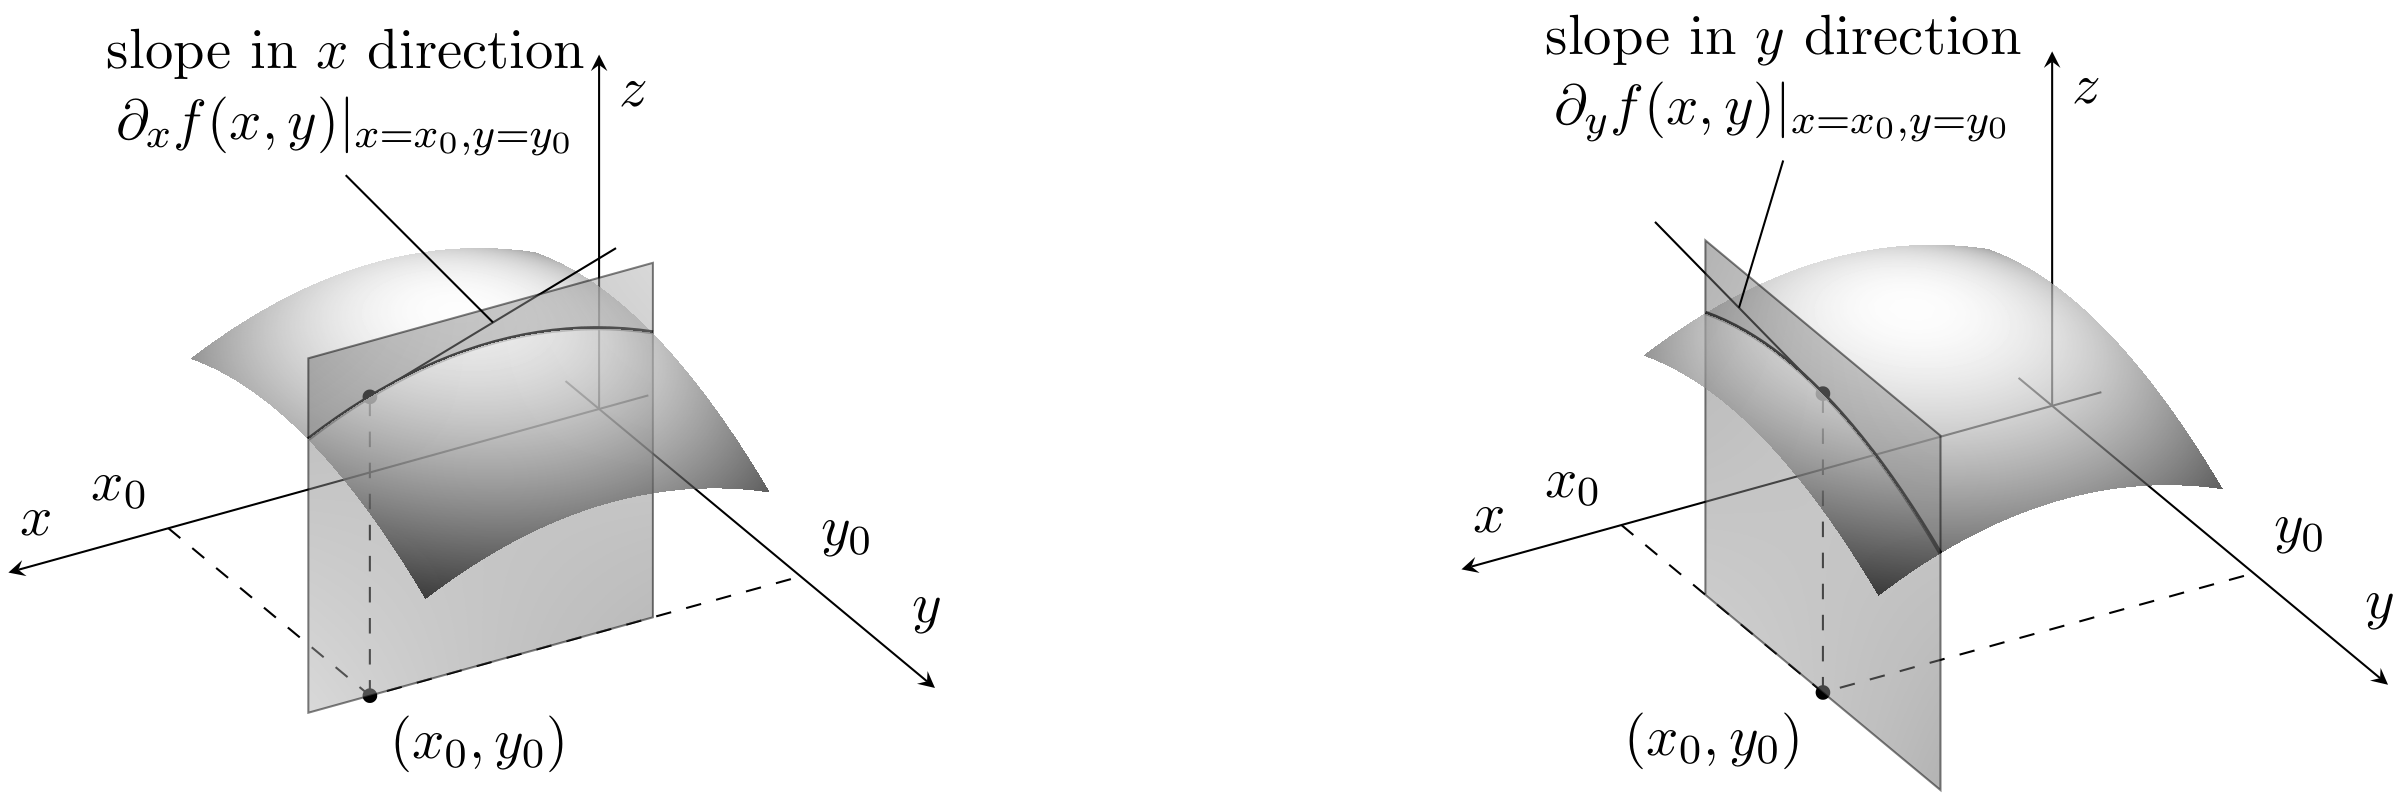
\includegraphics[width=0.9\textwidth]{derivate-parziali-significato-geometrico.png}
          \vspace{4mm}

          Questi due coefficienti angolari sono quelli delle rette tangenti al grafico che stanno sulla rispettiva traccia e che sono inoltre passanti per il punto \((x_0,y_0,f(x_0,y_0))\).

          Il piano formato dalle due rette rappresenta il piano tangente alla funzione nel punto \((x_0,y_0)\), ed ha equazione:

          \[
              z = f(x_0,y_0) + f_x(x_0,y_0) (x-x_0) + f_y(x_0,y_0) (y-y_0)
          \]
\end{itemize}

\subsubsection*{Esempio}

Scrivere l'equazione del piano tangente alla funzione \(z = x^{2}+y^{2}\) in \(P_0=(1,2)\),
dove \((x,y,z) \in S\), con \(S\) il grafico della funzione \(f(x,y)\).

Usando l'equazione del piano tangente:
\[
    P_0=(1,2) \iff (1,2,5) \in S
\]
\[
    z= 5+ 2(x-1) + 4(y-2) = 2x+4y -5
\]
quindi l'equazione richiesta è:
\[
    z = 2x+4y-5
\]

Vediamolo graficamente:
\filbreak{}

\begin{center}
    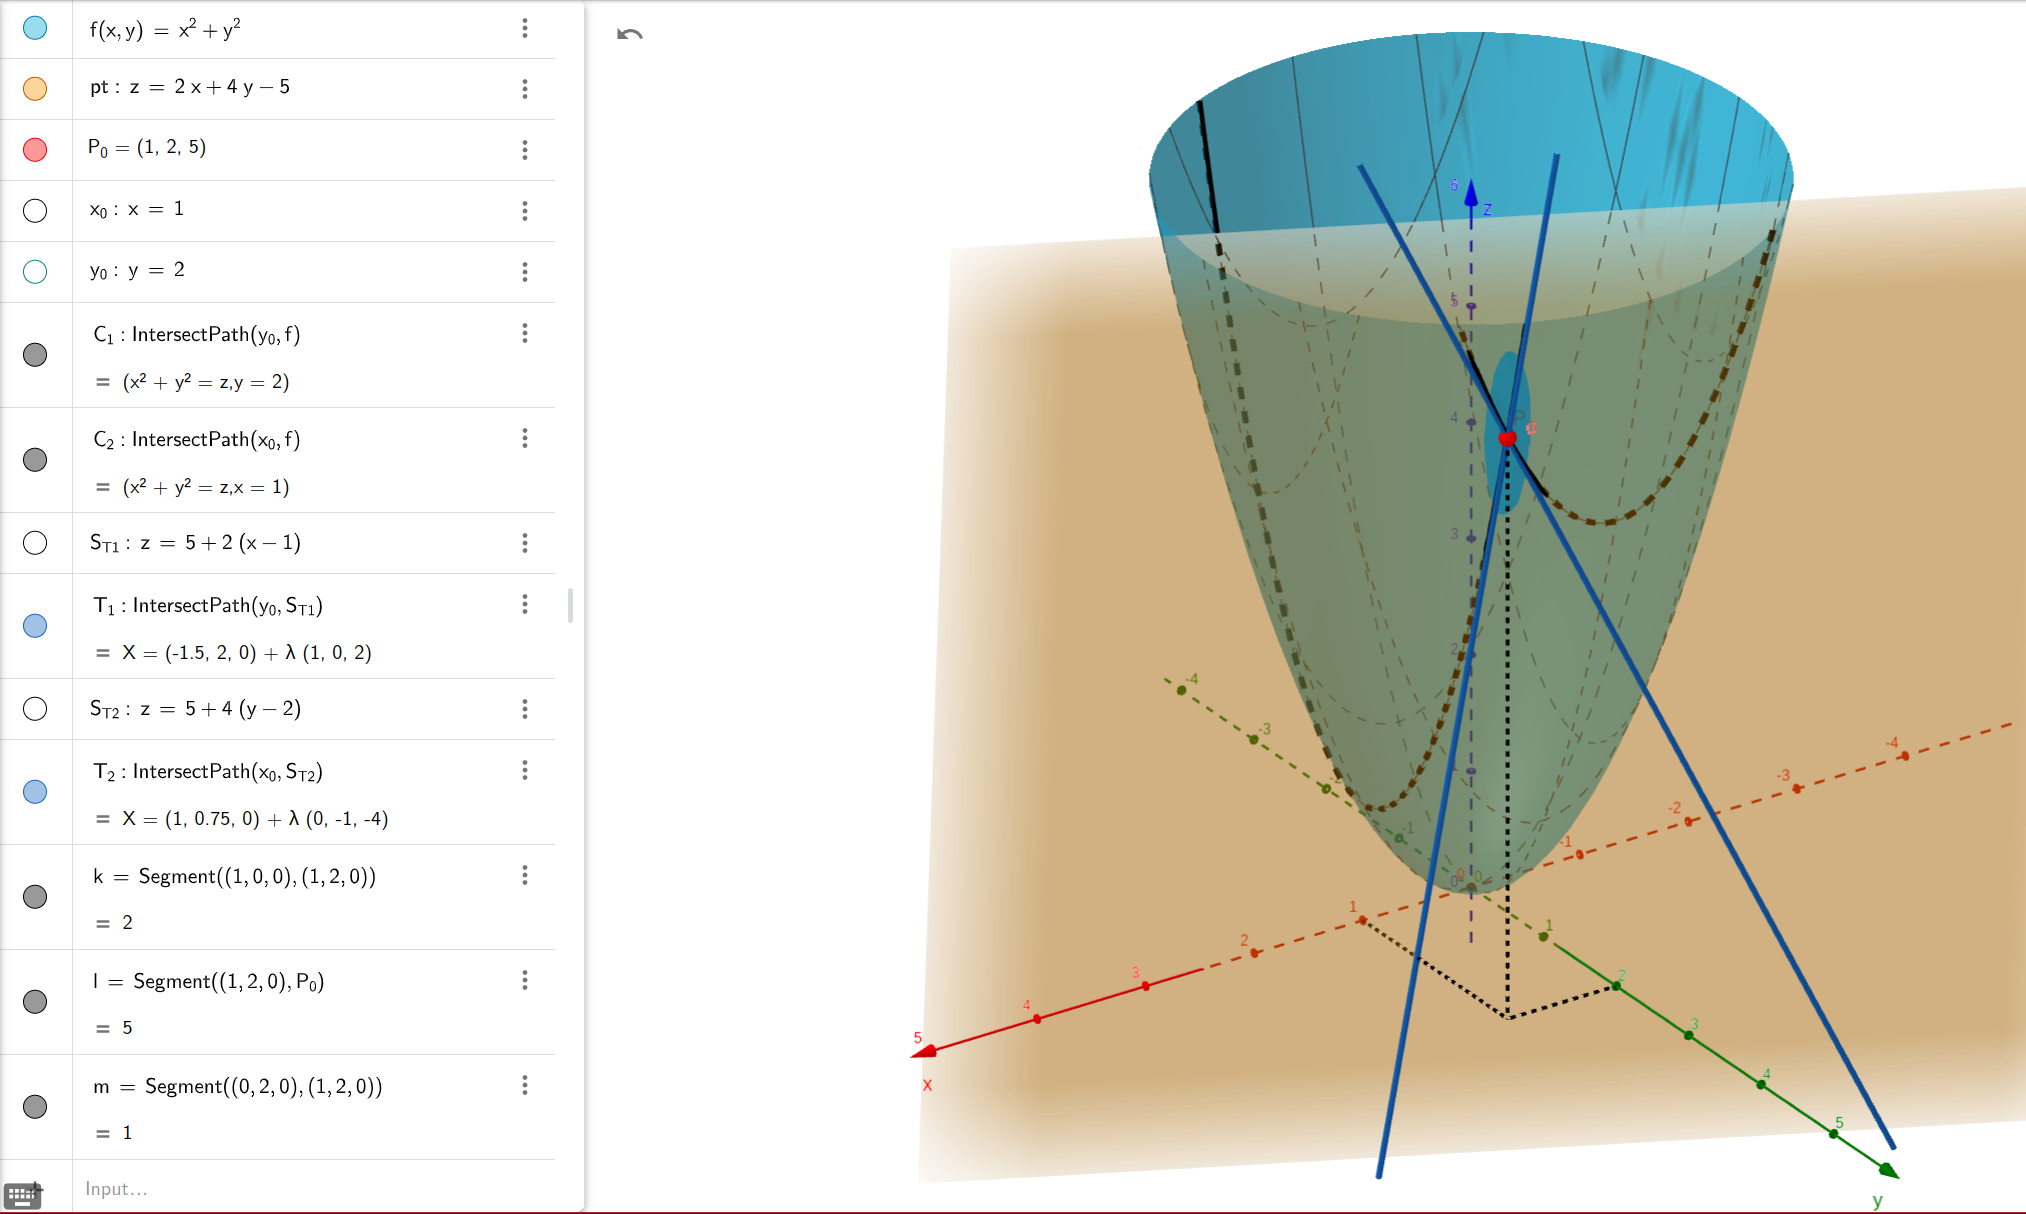
\includegraphics[width=0.79\textwidth]{piano-tangente-1.png}
    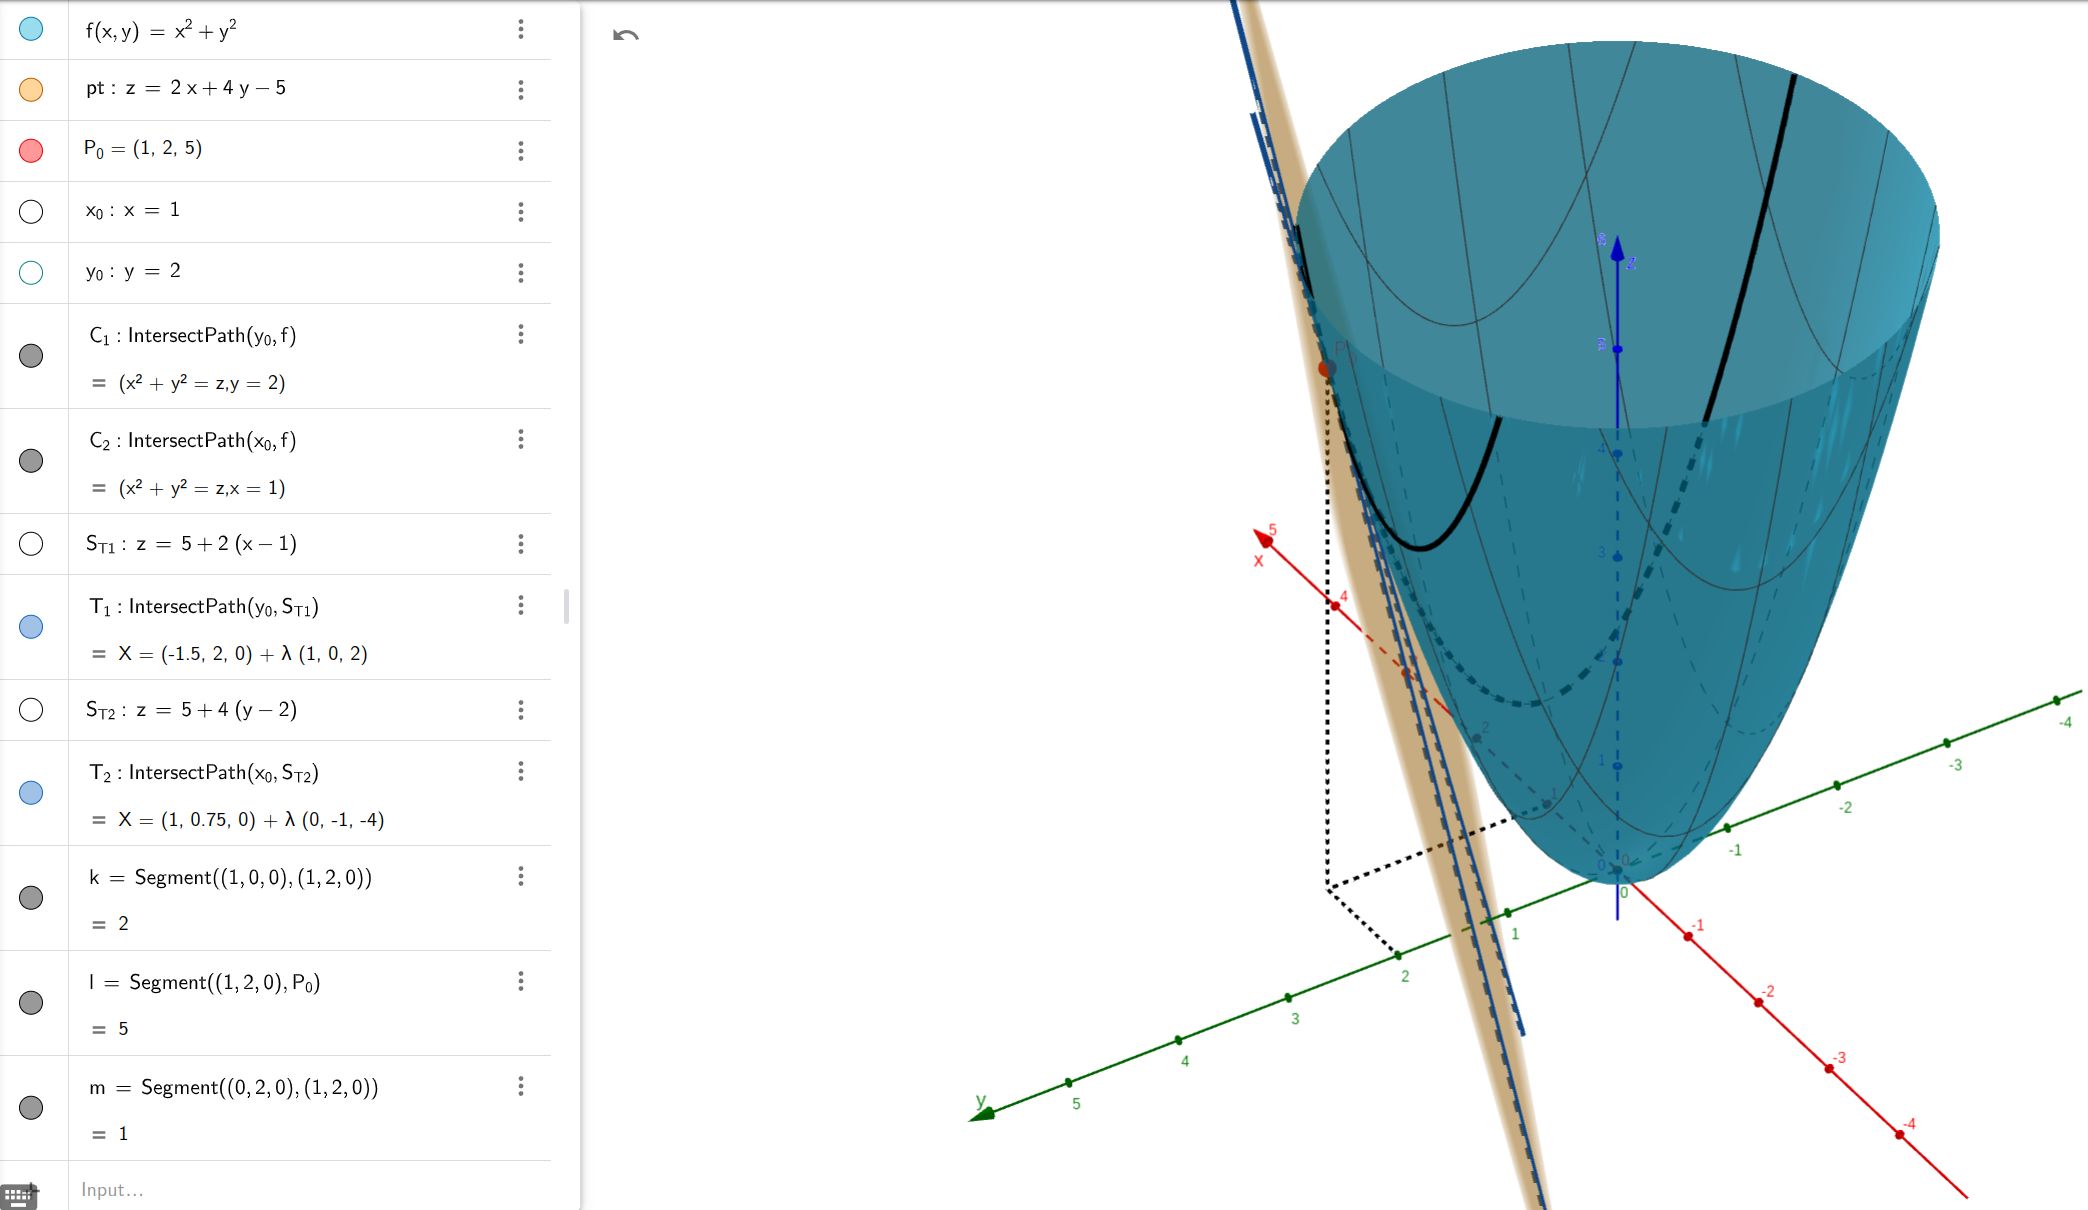
\includegraphics[width=0.79\textwidth]{piano-tangente-2.png}
    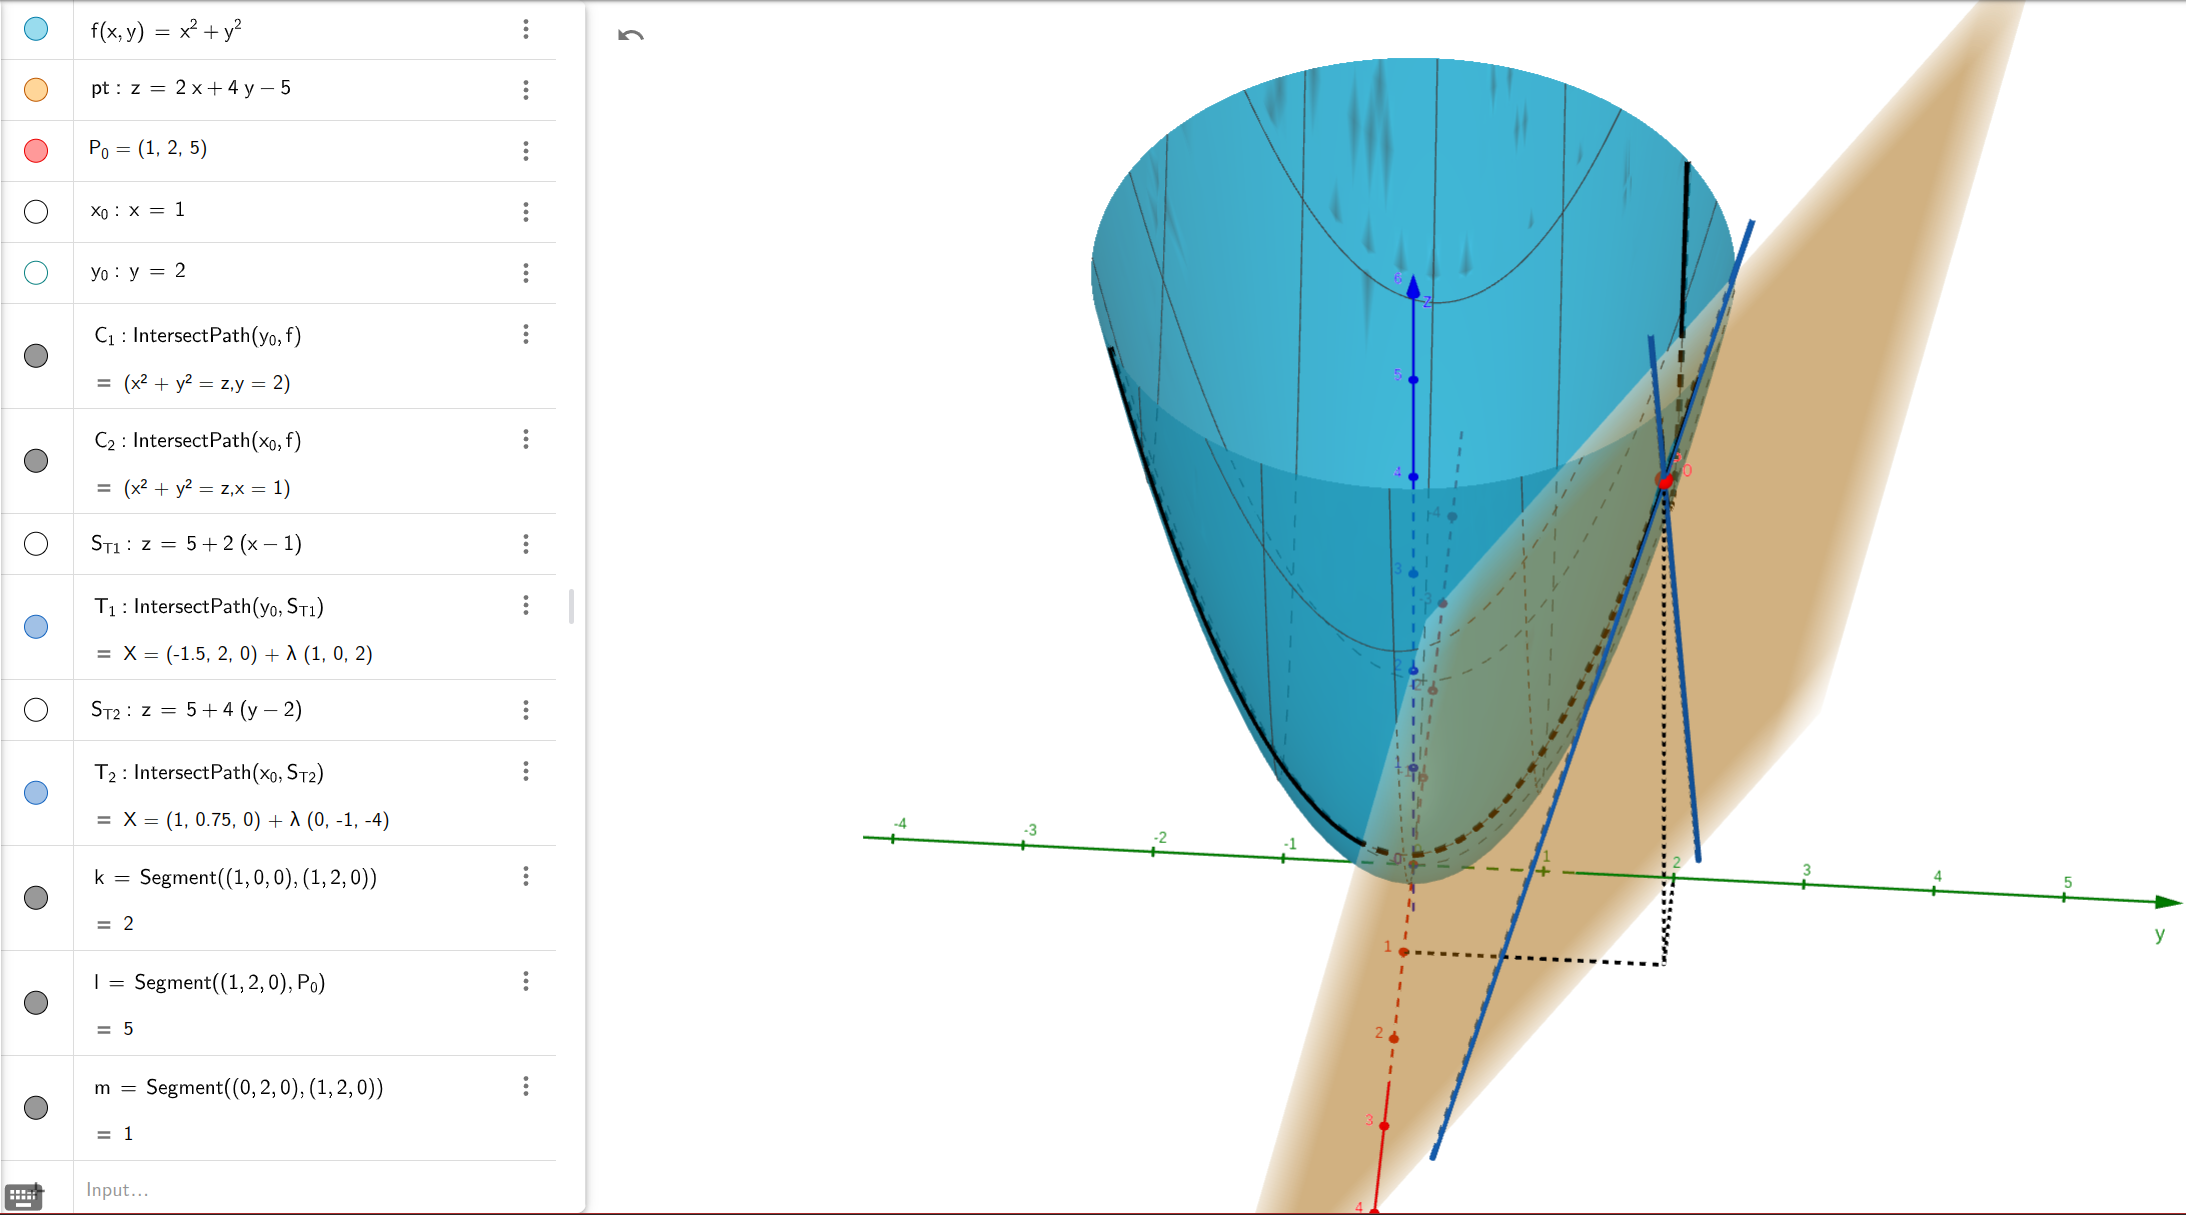
\includegraphics[width=0.79\textwidth]{piano-tangente-3.png}
\end{center}

\filbreak{}
\subsubsection{Definizione di derivabilità con il vettore gradiente}

Sia \(f: A \subset \R^2 \to \R \);

\(f\) si dice derivabile in \(A\) se esistono \(\frac{\partial f}{\partial x}\) e \(\frac{\partial f}{\partial y}\) in ogni punto di \(A\).

Ovvero, se esiste il \textbf{vettore gradiente}:

\[
    \nabla f(x,y)=\left( \frac{\partial f}{\partial x}(x,y), \frac{\partial f}{\partial y}(x,y) \right) \in \R^2
\]

Il vettore gradiente di \(f\) in \((x_0, y_0)\) è un vettore.

\textbf{In generale}:

In generale, per \(n\) variabili:

Data \(f: A \subset \R^n \to \R \), e \(\ux = (x_1, \ldots, x_n)\);

\(f\) è derivabile in \(\ux \in A\) se:

\[\exists \frac{\partial f}{\partial x_i}(\ux) ~\forall i = 1,\ldots,n\]

Ovvero se esiste finito il vettore gradiente:
\[
    \nabla f(\ux ) = \left( \frac{\partial f}{\partial x_1}\left(\ux\right), \frac{\partial f}{\partial x_2}\left(\ux\right), \ldots , \frac{\partial f}{\partial x_n}(\ux ) \right) \in \Rn
\]

\filbreak{}
\subsubsection{Derivata direzionale}

La derivata parziale è possibile scriverla anche secondo un'altra notazione. Partendo dalla notazione standard vista fino a ora:

\[
    f_{x_i} (\ux ) = \frac{\partial f}{\partial x_i}(\ux )
\]

definisco un \textbf{versore}, ovvero un vettore di modulo 1, nel modo seguente \(\forall i = 1, \ldots ,n\):

\[
    \underline{e_i} = (0, \ldots 0,1,0,\ldots,0)
\]

quindi, posso dire che la derivata parziale è data dal seguente limite, purché esista e sia finito:

\[
    \lim_{ h \to 0 } \frac{f(\ux + h \underline{e_i}) - f(\ux )}{h} = f_{x_i}(\ux )
\]

dove \(\ux + h \underline{e_i} = (x_1, \ldots, x_i, \ldots, x_n) + (0,\ldots,0,h,0,\ldots,0)\) è la \textbf{notazione vettoriale} di \(\ux \).

Dunque, espandendo:

\[
    f( \ux +h \underline{e_i} ) = f( x_{1}, \ldots , x_{i-1},x_{i}+h , x_{i+1}, \ldots ,x_{n})
\]

vediamo che dipende solo da h; quindi la derivata direzionale di \(f\) nella direzione di \(\underline{e_i}\) è la derivata della funzione di 1 variabile:

\[
    g(h) = f(\ux + h \underline{e_i} )
\]

Se g è derivabile in \(h=0\), allora:

\[
    g'(0) = \frac{\partial f}{\partial x_i}(\ux ) = f_{x_i}(\ux)
\]

ovvero significa che esiste, finito, il limite:

\[
    g'(0) = \lim_{ h \to 0 } \frac{g(h) - g(0)}{h-0} = \lim_{ h \to 0 } \frac{f(\ux +h \underline{e_i} ) - f(\ux )}{h} = \frac{\partial f}{\partial x_i}(\ux)
\]

\subsubsection*{Generalizzazione}

Se abbiamo \(\vec{v} \), una direzione in \(\Rn \) di modulo 1, ovvero \(\vec{v}\) versore in \(\Rn \):

\[
    \norm{\vec{v}} = \sqrt{\sum^{n}_{i=1} {v_i}^{2}} = 1
\]

Allora, definisco la \textbf{derivata direzionale} come:

\[
    \frac{\partial f}{\partial \vec{v}}(\ux) = D_{\vec{v}} f(\ux ) = \lim_{ h \to 0 } \frac{f(\ux +h \vec{v} ) -f(\ux )}{h}
\]

\filbreak{}
\subsubsection*{Per n=2}

Se prendiamo un punto \(P_0 = (x_0, y_0)\), le due derivate direzionali saranno:
\begin{align*}
    \frac{\partial f}{\partial x}(P_0) = \text{derivata parziale di f nella direzione di } e_1 = \text{asse } x \\[3mm]
    \frac{\partial f}{\partial y}(P_0) = \text{derivata parziale di f nella direzione di } e_2 = \text{asse } y
\end{align*}

\subsubsection*{Per n=3}

Sia \(f: A \subseteq \R^{3} \rightarrow \R \) una funzione;

Consideriamo \(\vec{v} = (a,b,c) \in \R^{3}\) come vettore direzionale. Vale quindi \(\norm{\vec{v}} =1\).

Calcoliamo la derivata direzionale rispetto a \(\vec{v}\), che è il seguente limite, se esiste, finito:

\[
    D_{\vec{v}} f(\ux ) = \lim_{ h \to 0 } \frac{f(\ux + h \vec{v} ) -f(\ux )}{h}
\]

dove \(\ux = (x_0,y_0,z_0)\), quindi:

\[
    D_{\vec{v}} f(\ux ) = \lim_{ h \to 0 } \frac{f(x_0+ha,y_0+hb,z_0+hc) - f(x_0,y_0,z_0)}{h}
\]

Quindi, se il limite esiste ed è finito, avremmo le 3 derivate parziali:
\begin{align*}
    \frac{\partial f}{\partial x}(\underline{P_0}) = f_x(\underline{P_0}) = D_{\vec{e_1}}f(\underline{P_0}) = \text{derivata parziale di f nella direzione di } \vec{e}_1 \\[3mm]
    \frac{\partial f}{\partial y}(\underline{P_0}) = f_y(\underline{P_0}) = D_{\vec{e_2}}f(\underline{P_0}) = \text{derivata parziale di f nella direzione di } \vec{e}_2 \\[3mm]
    \frac{\partial f}{\partial z}(\underline{P_0}) = f_z(\underline{P_0}) = D_{\vec{e_3}}f(\underline{P_0}) = \text{derivata parziale di f nella direzione di } \vec{e}_3
\end{align*}

dove, \(\vec{e}_1, \vec{e}_2, \vec{e}_3\) sono i versori degli assi \(x,y,z\), ovvero:
\begin{align*}
     & \vec{e}_1 = (1,0,0) = \vec{i} \\
     & \vec{e}_2 = (0,1,0) = \vec{j} \\
     & \vec{e}_3 = (0,0,1) = \vec{w}
\end{align*}

\subsubsection*{Conclusione}

Per concludere, dire che \(f\) è derivabile in \(P_0 \in \Rn \) equivale a dire che esiste il vettore gradiente:

\[
    \Rn \ni \nabla f(\ux) = \left( \frac{\partial f}{\partial x_1}(\ux), \ldots, \frac{\partial f}{\partial x_n}(\ux) \right)
\]

con \(x_i\) tutte le varie direzioni.
